\section{Expérience C3} 
  \subsection{Objectif}
    Comprendre de quelles manières un réseau de neurone connexionniste peut parier sur ses propres résultats
    à partir de ses représentations personnelles.

    
    Réalisation de la seconde expérience de l'article \cite{Cleeremans_2007} sur des données réelles
    non linéairement séparables.
  
  
  \subsection{Architecture}
    \paragraph{Description}
      Un premier réseau de perceptron multicouche apprend à discrétiser des fleurs caractérisées
      par 4 neurones d'entrées qui représentent taille et largeur de la pétale et la sépale. 
      Il est composé d'une couche cachée de 5 ou 100 neurones.
      
      Un second réseau de perceptron multicouche apprend à parier sur la qualité de la réponse
      du premier réseau à partir de sa couche cachée.
      
      L'apprentissage du second réseau, n'affecte pas les poids entre la couche d'entrée et la 
      couche cachée du premier réseau.

    \paragraph{Schéma}
      \begin{center}
	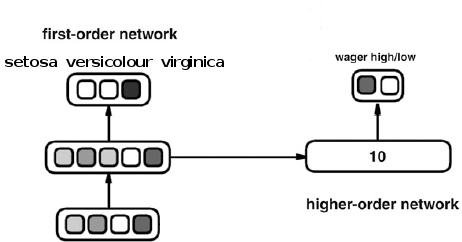
\includegraphics[width=230px]{data/expC3/schema.png}
      \end{center}
      
    \paragraph{Paramètres}
      \begin{center}
	\begin{tabular}{lr}
	  \begin{minipage}{230px}
	    \begin{itemize}
	      \item momentum : 0.5 sur le premier réseau
	      \item momentum : 0. sur le second réseau
	      \item taux d'apprentissage : 0.15 sur les 2 réseaux
	      \item \textbf{150 formes} de fleurs différents présentées (shuffle) \cite{Iris}
	      \item apprentissage 50 (formes) x 300 (époques)
	      \item utilisation de biais
	      
	    \end{itemize}
	  \end{minipage}
	  &
	  \begin{minipage}{230px}
	    \begin{itemize}
	      \item poids initialisés sur [-1 ; 1] pour le premier réseau
	      \item poids initialisés sur [-0.25 ; 0.25] pour le second réseau
	      \item taux d'apprentissage constant
	      \item entrées réelles sur [0 ; 1]
	      \item sigmoïde à température 1
	    \end{itemize}
	  \end{minipage}
	\end{tabular}
      \end{center}

  
  \newpage
  \subsection{Résultats}
    \paragraph{Principaux}
      Analyse des performances
      \begin{center}
	\begin{tabular}{lr}
	  \hspace*{-1cm}
	  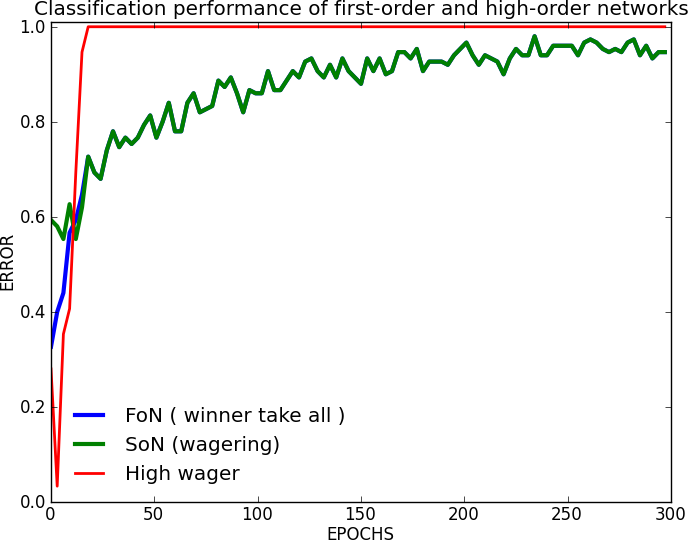
\includegraphics[width=250px]{data/expC3/perf_5.png}
	  &
	  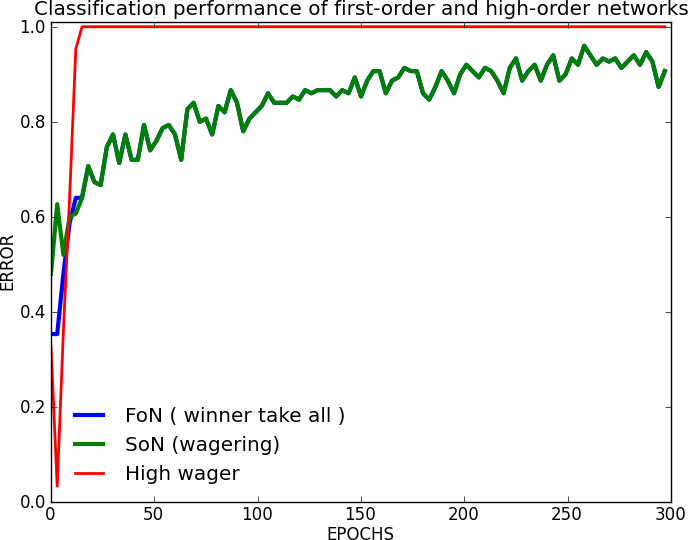
\includegraphics[width=250px]{data/expC3/perf_100.png} 
	\end{tabular}
      \end{center}
      \subparagraph{Notes}
	\begin{itemize}
	  \item la performance de classification représente le taux de bonnes réponses (winner-take-all) pour les 50 formes présentées sur une époque
	  \item la courbe rouge représentent le taux de paris hauts du second réseau
	\end{itemize}
      \subparagraph{Conclusion}
	\begin{itemize}
	  \item dans les 2 cas, le premier réseau réussit à apprendre sa tâche de classification
	  \item dans les 2 cas, le second réseau n'arrive pas à tirer parti de ses représentations, 
	  il se contente simplement de parier haut au bout d'un moment
	\end{itemize}
    \paragraph{Secondaires}
      RMS
      \begin{center}
	\begin{tabular}{lr}
	  \hspace*{-1cm}
	  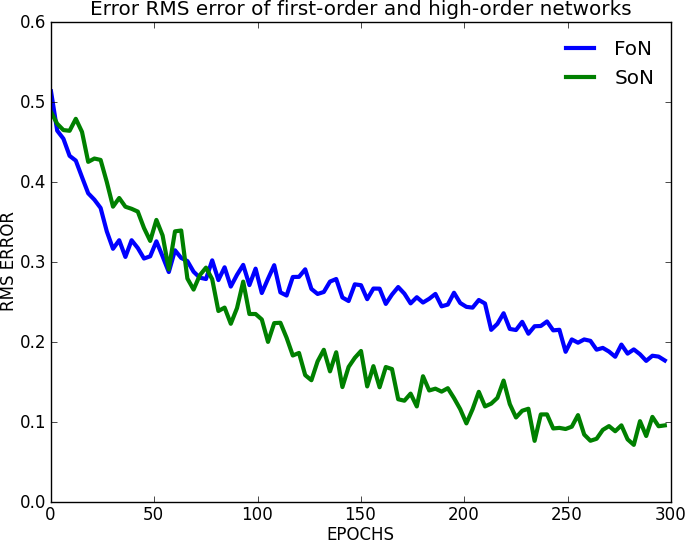
\includegraphics[width=250px]{data/expC3/rms_5.png}
	  &
	  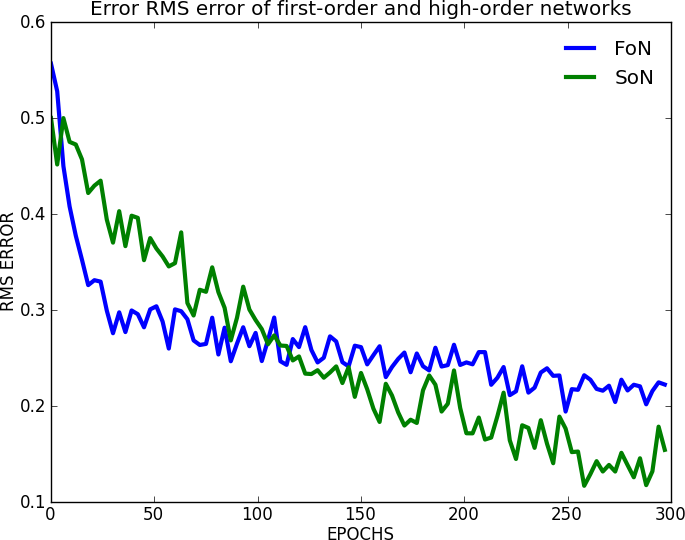
\includegraphics[width=250px]{data/expC3/rms_100.png} 
	\end{tabular}
      \end{center} 
      \subparagraph{Notes}
	\begin{itemize}
	  \item formule utilisée pour RMS (cf. Formules~\nameref{rms})
	\end{itemize}
      \subparagraph{Conclusion}
	Il n'y a plus de pique du second réseau comme dans les \nameref{expC1} et \nameref{expC2}.


  \subsection{Conclusion}
        Comme il l'est dit dans \cite{Cleeremans_2007}, cette architecture de résoudre les problèmes des réseaux connexionnistes
    classiques à avoir un semblant de conscience.
    
    À savoir :
    \begin{itemize}
    \item qu'ils ne savent pas qu'ils peuvent se trouver dans différents états, et qu'ils ne traitent pas leurs propres états : 
    d'où la présence de ce second réseau qui tente de traiter ses états et d'apprendre qu'il en a plusieurs
    \item des représentations rentant bloquées dans la chaîne de causalité de la tâche à apprendre : d'où
    le fait que ce second réseau n'affecte pas l'apprentissage du premier (ie. pour ne pas retomber dans la chaîne de causalité)
    \item qu'ils n'ont pas les connaissances conscientes des raisons de leurs décisions : on essaye de les y sensibiliser avec les paris
    \\[0.2cm]
    \end{itemize}
  
    Lors du passage sur des données réelles non linéairement séparables, l'utilité du second réseau
    s'écroule, les représentations ne sont plus exploitées.
    
    Pour tenter de résoudre ce problème, l'\nameref{expC4} augmente le nombre de couche du premier réseau.

  \newpage 
  \subsection{Formules}
    \paragraph{RMS} \label{rms}
  Pour une époque $e$ :
  \begin{center}
    \begin{large}
    $ rms_{e} = \sqrt{ \frac{1}{n} \sum \limits_{i=1}^{n} 
    ( o_{i,e} - d_{i} )^2 } $
    \end{large}
  $ with \left\lbrace \begin{array}{lll} n : number\ of\ neurons\ on\ the\ output\ 
  layer\\o_{i,e} : value\ obtained\ for\ the\ i^{th}\ neuron\ at\ the\ e^{th}\ epoch\\d_{i} : 
  value\ desired \ for\ the\ i^{th}\ neuron\end{array} \right.$
  \end{center}
    \paragraph{Descente de gradient} \cite{Touzet_1992} \\
  Construction de l'erreur : 
    \begin{center}
      $y_{i} = f'(a_i) \times ( d_i - x_i ) \ si\ i\ neurone\ de\ sortie $ \\
      $y_{i} = f'(a_i) \times \sum \limits_{k} ( w_{ki} \times y_k )\ si\ i\ neurone\ cache $
    \end{center}
  Mise à jour des poids :
    \begin{center}
      $w_{ij}(t+1) = w_{ij}(t) + learning\_rate \times y_{i} \times x_j + momentum \times 
      (w_{ij}(t) - w_{ij}(t-1) )$
    \end{center}
  Variables : 
    \begin{center}
      $\left\lbrace \begin{array}{lll} 
	f : fonction\ sigmoide \\
	x_i : valeur\ du\ neurone\ i\\
	d_i : valeur\ desire pour\ le\ neurone\ i\\
	a_i : somme\ pondere\ des\ poids\ du\ neurone\ i
      \end{array} \right.$
    \end{center}
    
\bibliographystyle{../pre-rapport/apalike}
\bibliography{../pre-rapport/biblio}
